\documentclass{beamer}
%
% Choose how your presentation looks.
%
% For more themes, color themes and font themes, see:
% http://deic.uab.es/~iblanes/beamer_gallery/index_by_theme.html
%
\mode<presentation>
{
  \usetheme{default}      % or try Darmstadt, Madrid, Warsaw, ...
  \usecolortheme{default} % or try albatross, beaver, crane, ...
  \usefonttheme{default}  % or try serif, structurebold, ...
  \setbeamertemplate{navigation symbols}{}
  \setbeamertemplate{caption}[numbered]
} 

\usepackage[english]{babel}
\usepackage[utf8x]{inputenc}
\usepackage{graphicx}

\title[Progress Report]{Progress Report Presentation}
\author{Artem Vasenin}
\institute{Predicting arbitrary events in competitive computer team games}
\date{\today}

\begin{document}

\begin{frame}
  \titlepage
\end{frame}



\section{Main}

\begin{frame}{Aim}

\begin{itemize}
  \item Predict statistics about games other than winrate.
  \item Improve winrate prediction using associated information. Standard ranking algorithms don't perform well for games where teams change frequently.
\end{itemize}
\begin{center}
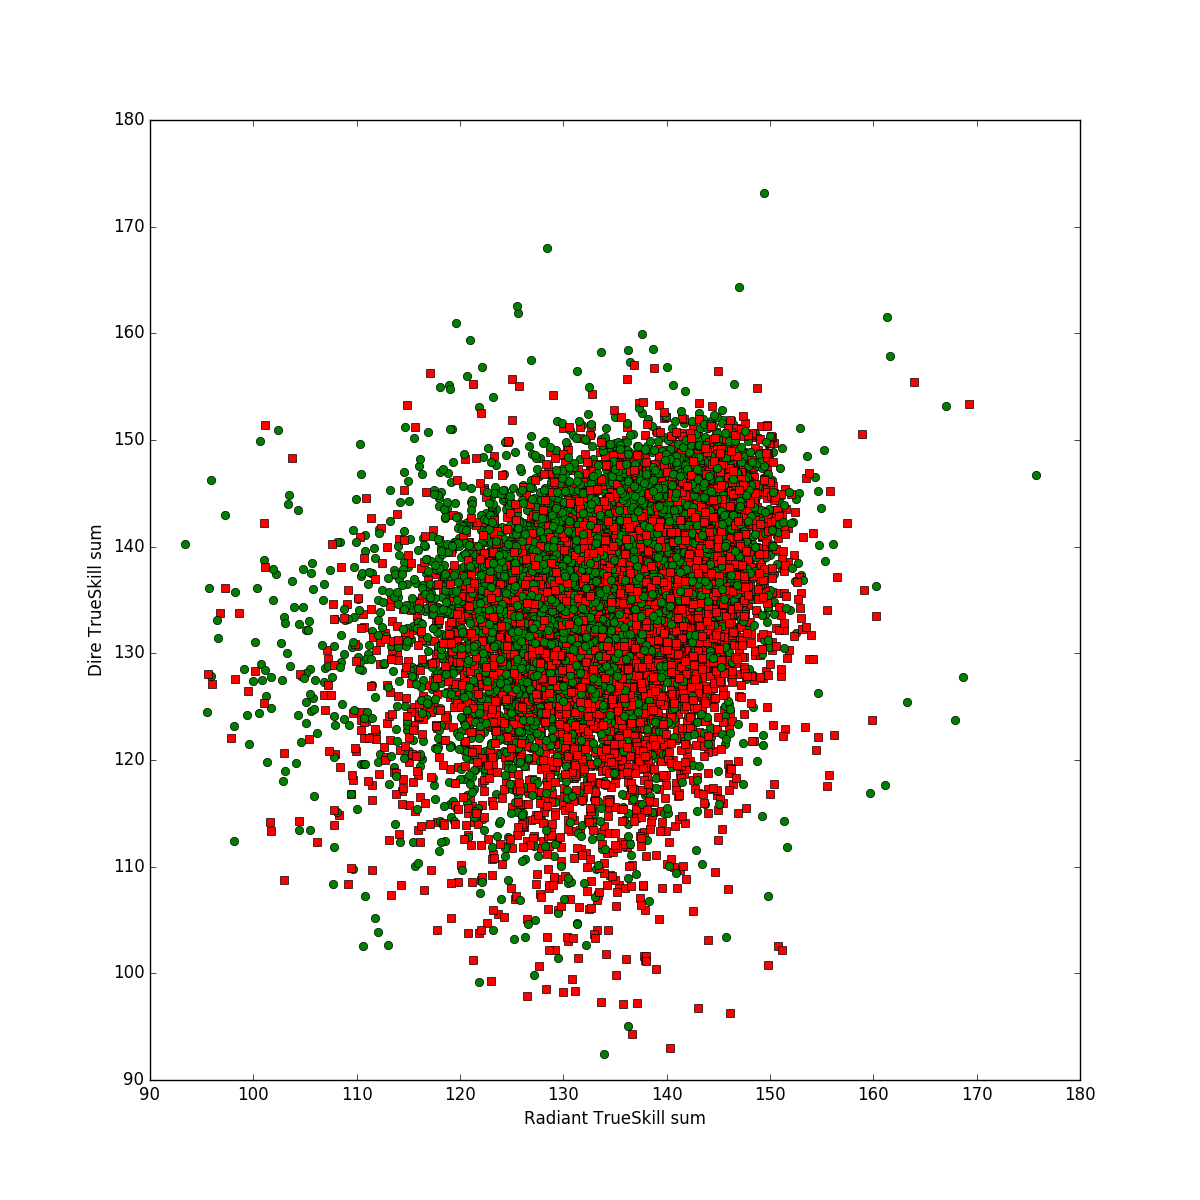
\includegraphics[width=6cm]{winrate}
\end{center}


\end{frame}

\begin{frame}{Algorithm Outline}
\begin{itemize}
\item Using raw data is inefficient since there is just too much of it.
\item Averages and other simple aggregation techniques don't work very well.
\item Need to create some representation of player's skill in different areas of the game. 
Use rating algorithms to approximate players skills.
\end{itemize}

\begin{enumerate}
\item Approximate players' skills using basic rating algorithms.
\item Train estimators using approximate skills.
\item Update approximations of players' skills using trained estimators.
\item Repeat 2 \& 3 until no further change.
\end{enumerate}

\end{frame}

\begin{frame}{Training}
Feature selection
\begin{itemize}
\item To improve computation speed and reduce over-fitting we can select features using forward pass.
\item Assume that player position is random within the team, therefore select features in groups. Each group being made up of the same skill of different players on the same team.
\end{itemize}
Types of estimation
\begin{itemize}
\item Regression, e.g.\ number of enemies killed, number of passes made
\item Excluding classification, e.g.\ win/loss
\item Non-excluding classification, e.g.\ items acquired by a player, red cards given to players.
\end{itemize}
Normalise non-excluding classification to get excluding one.
\end{frame}


\begin{frame}{Results}
\begin{center}
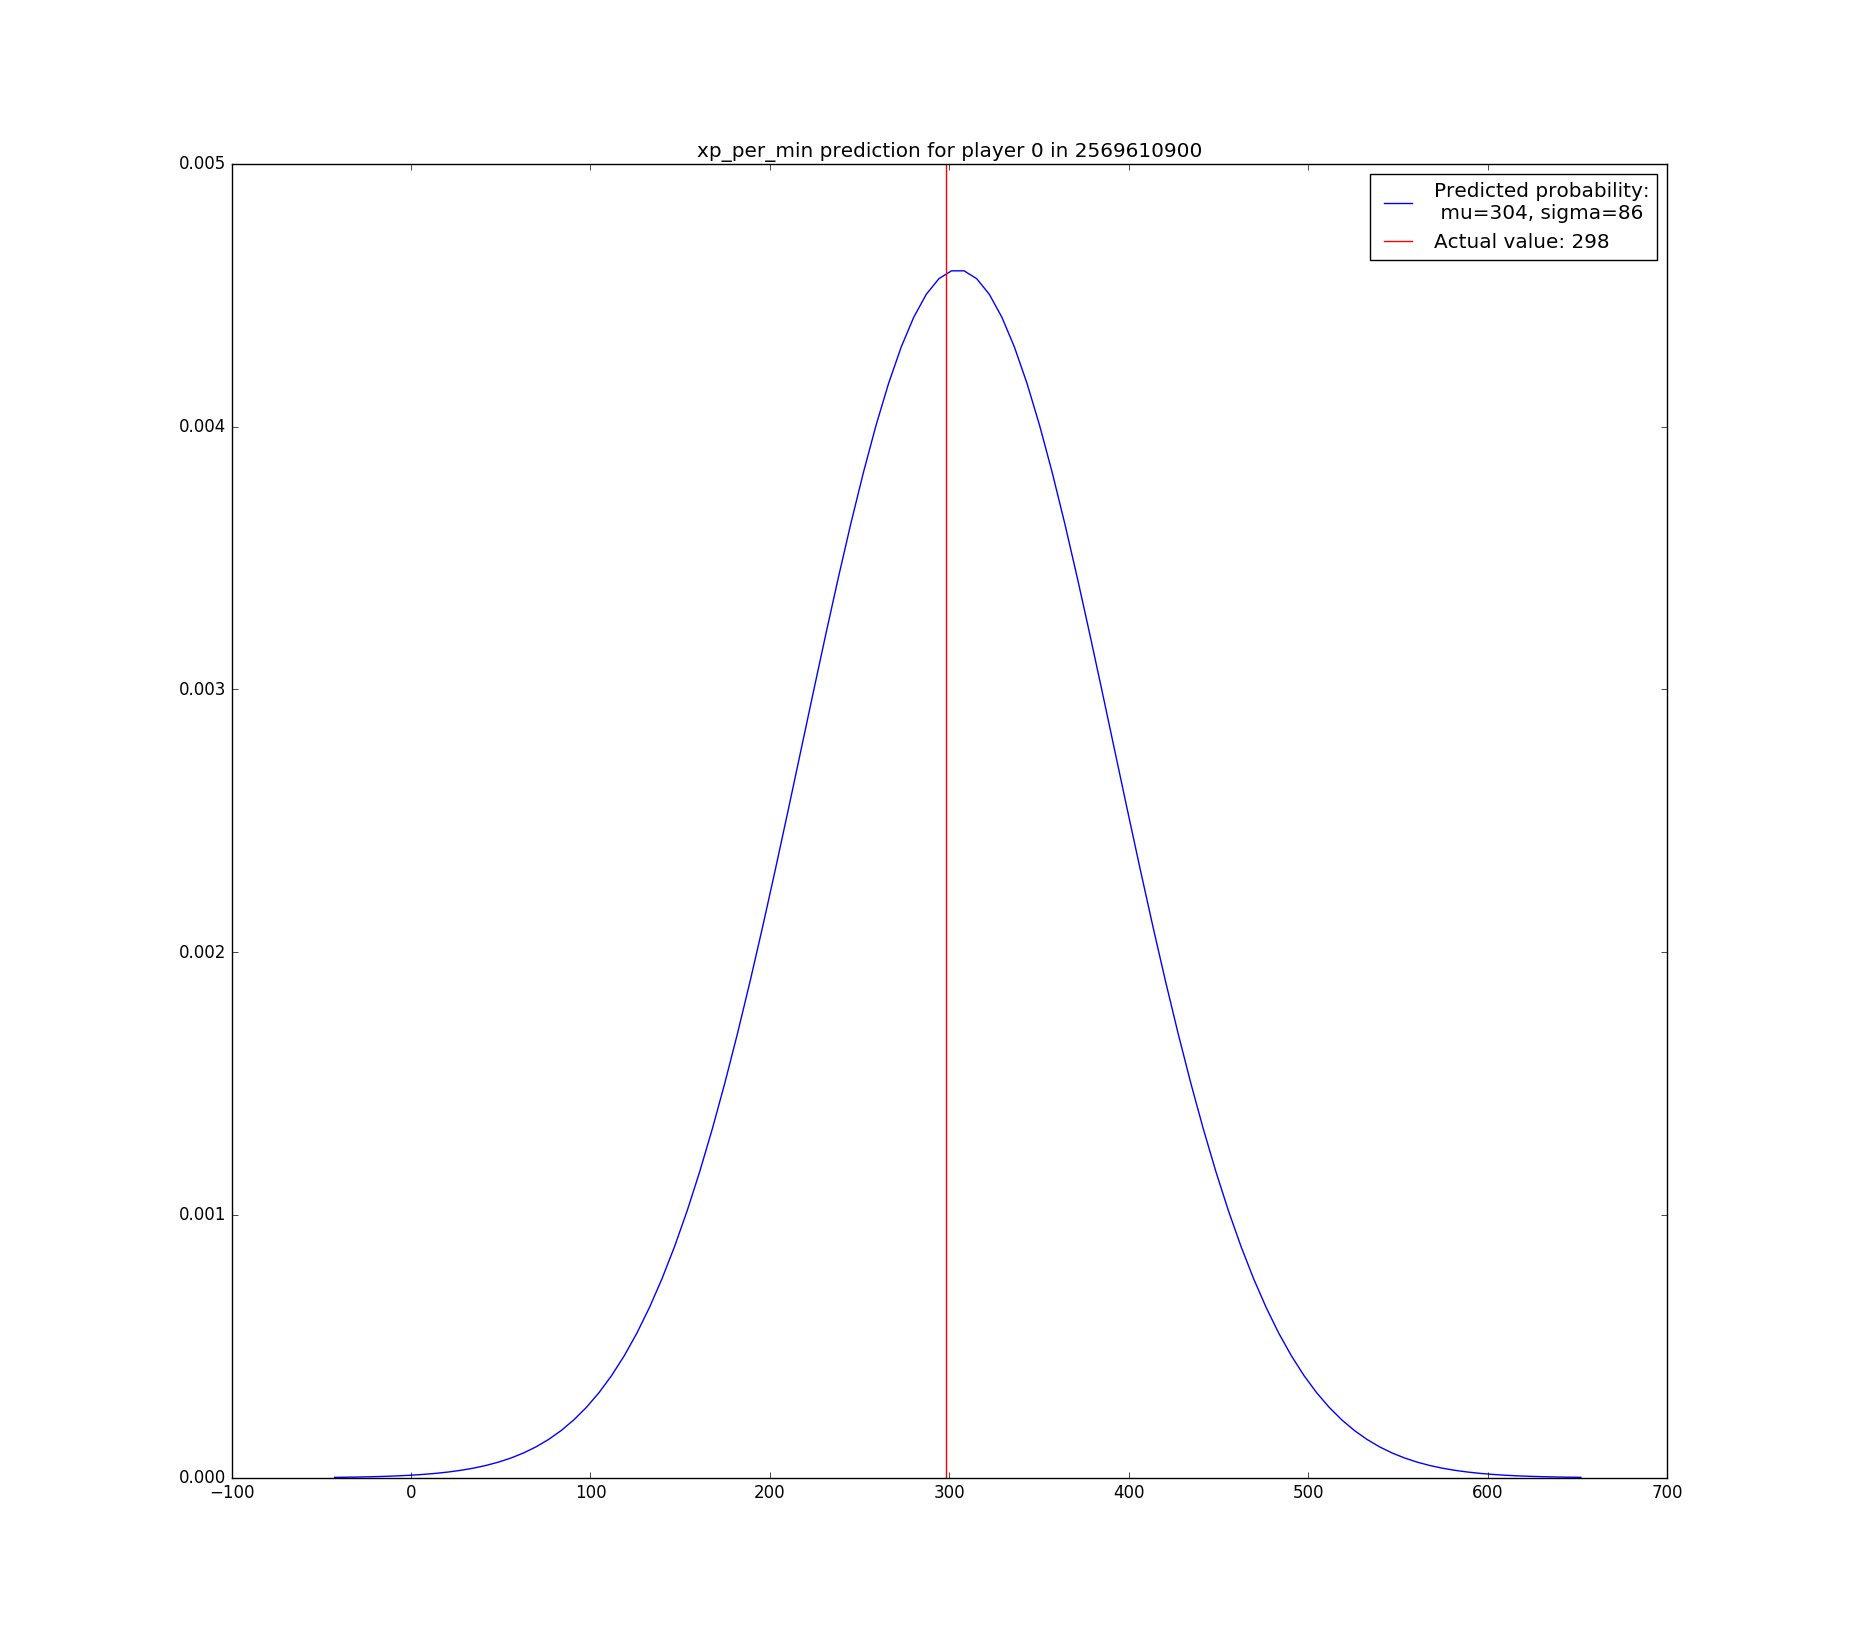
\includegraphics[width=5cm,height=4cm]{XPM_player_0_TI}
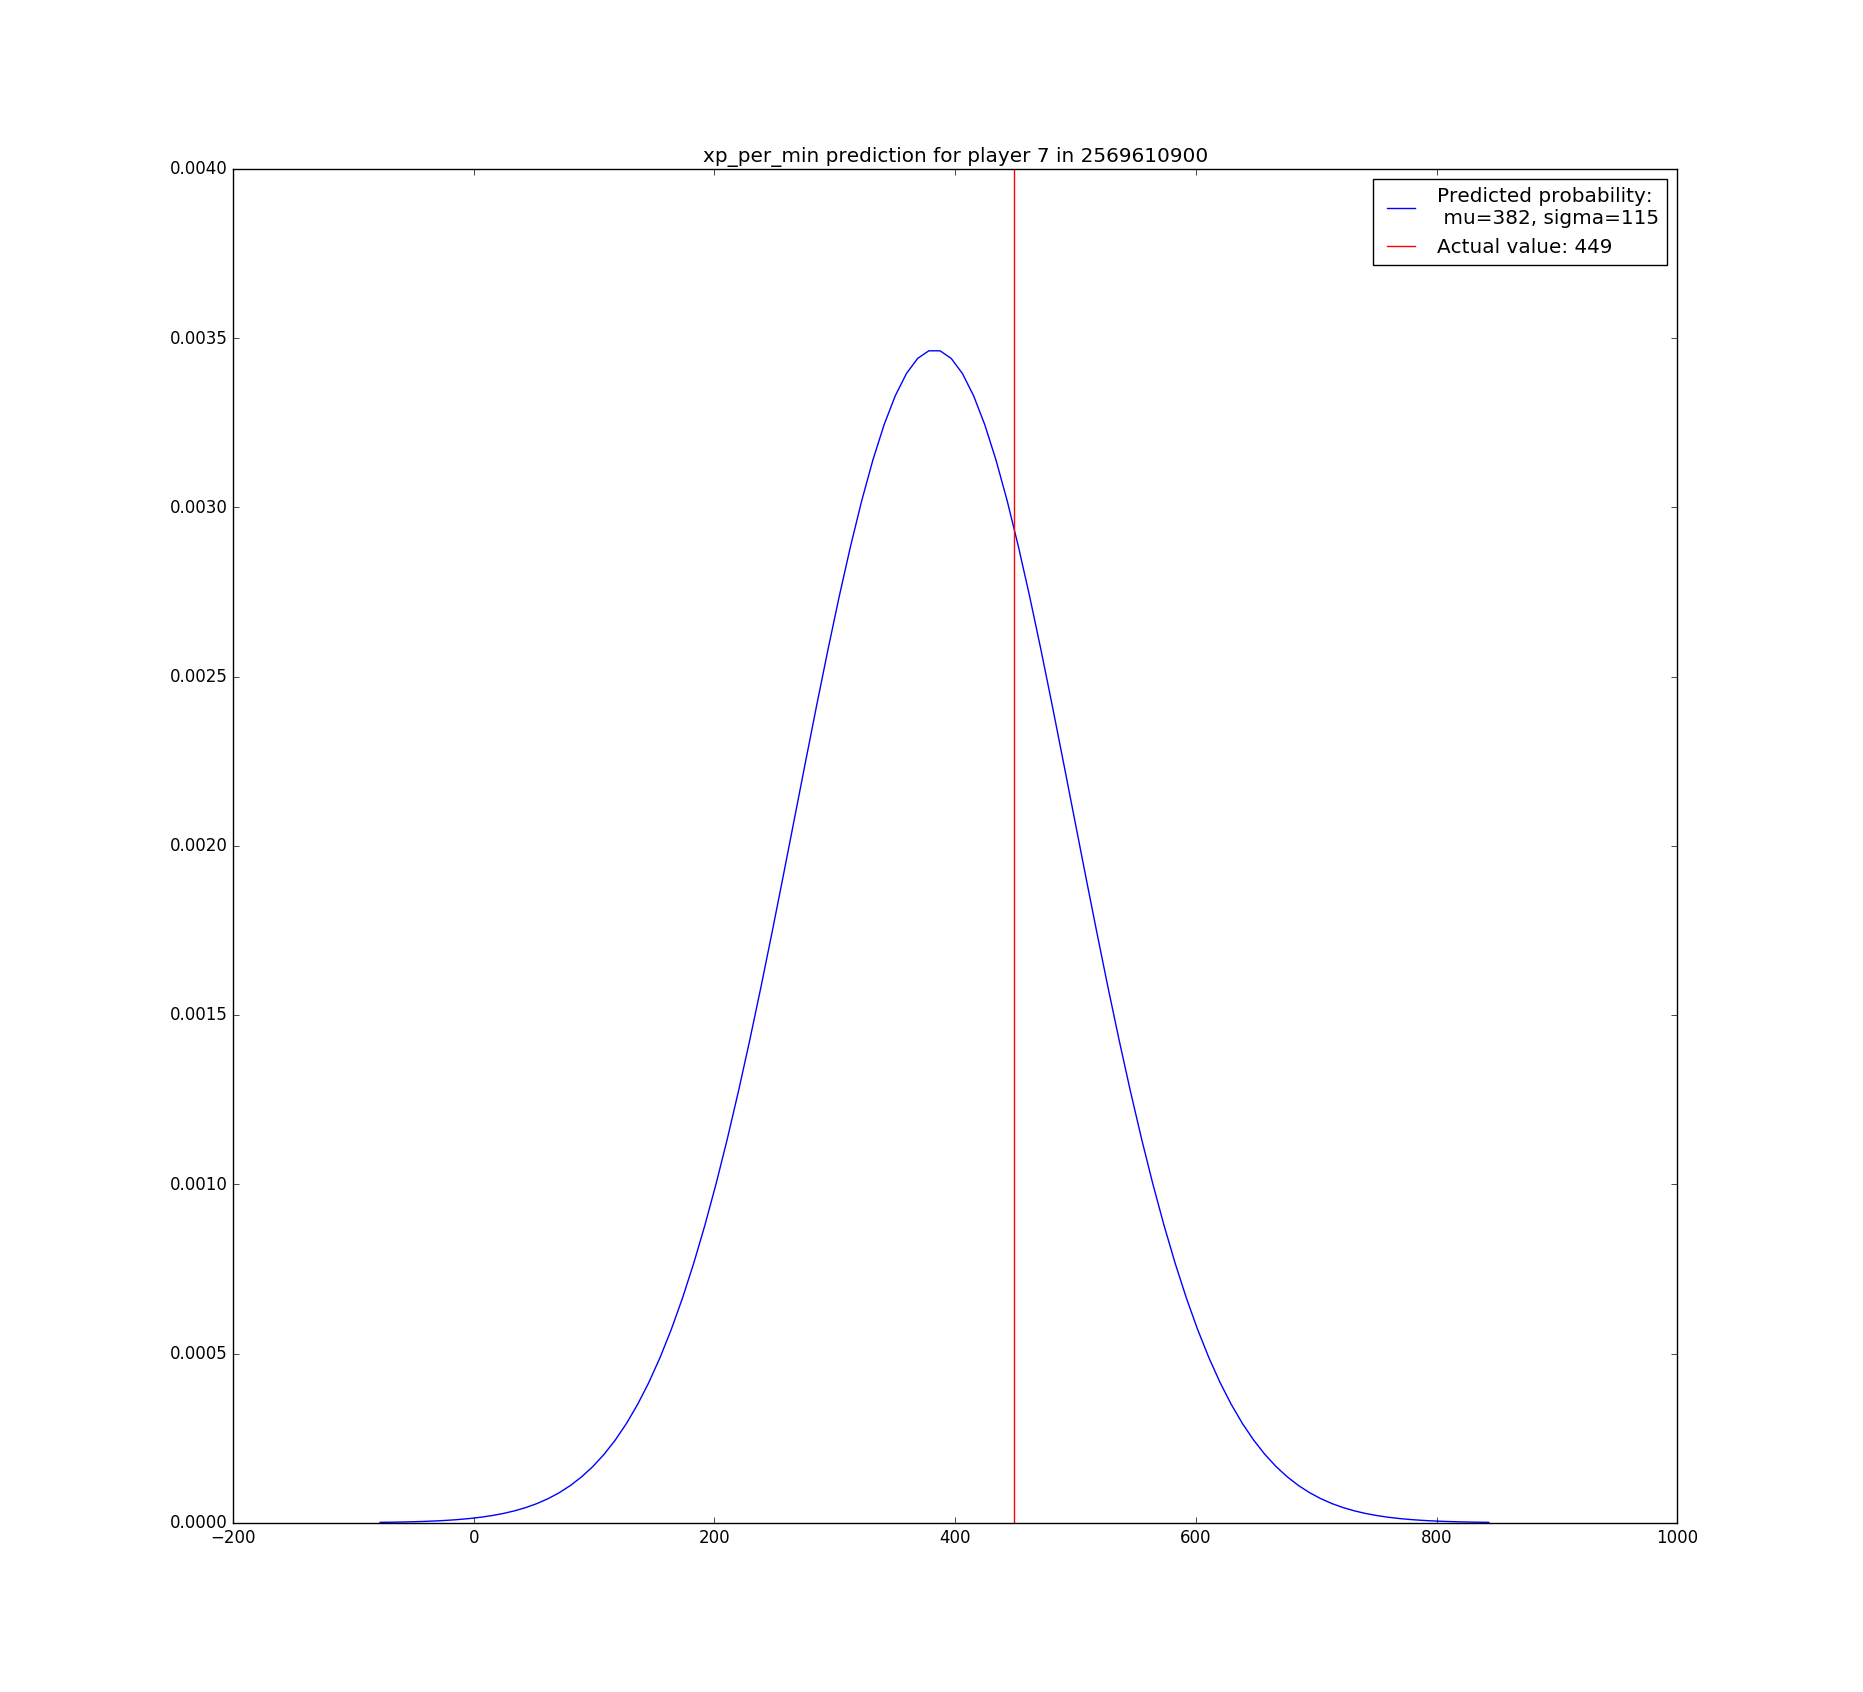
\includegraphics[width=5cm,height=4cm]{XPM_player_7_TI}
\newline{}
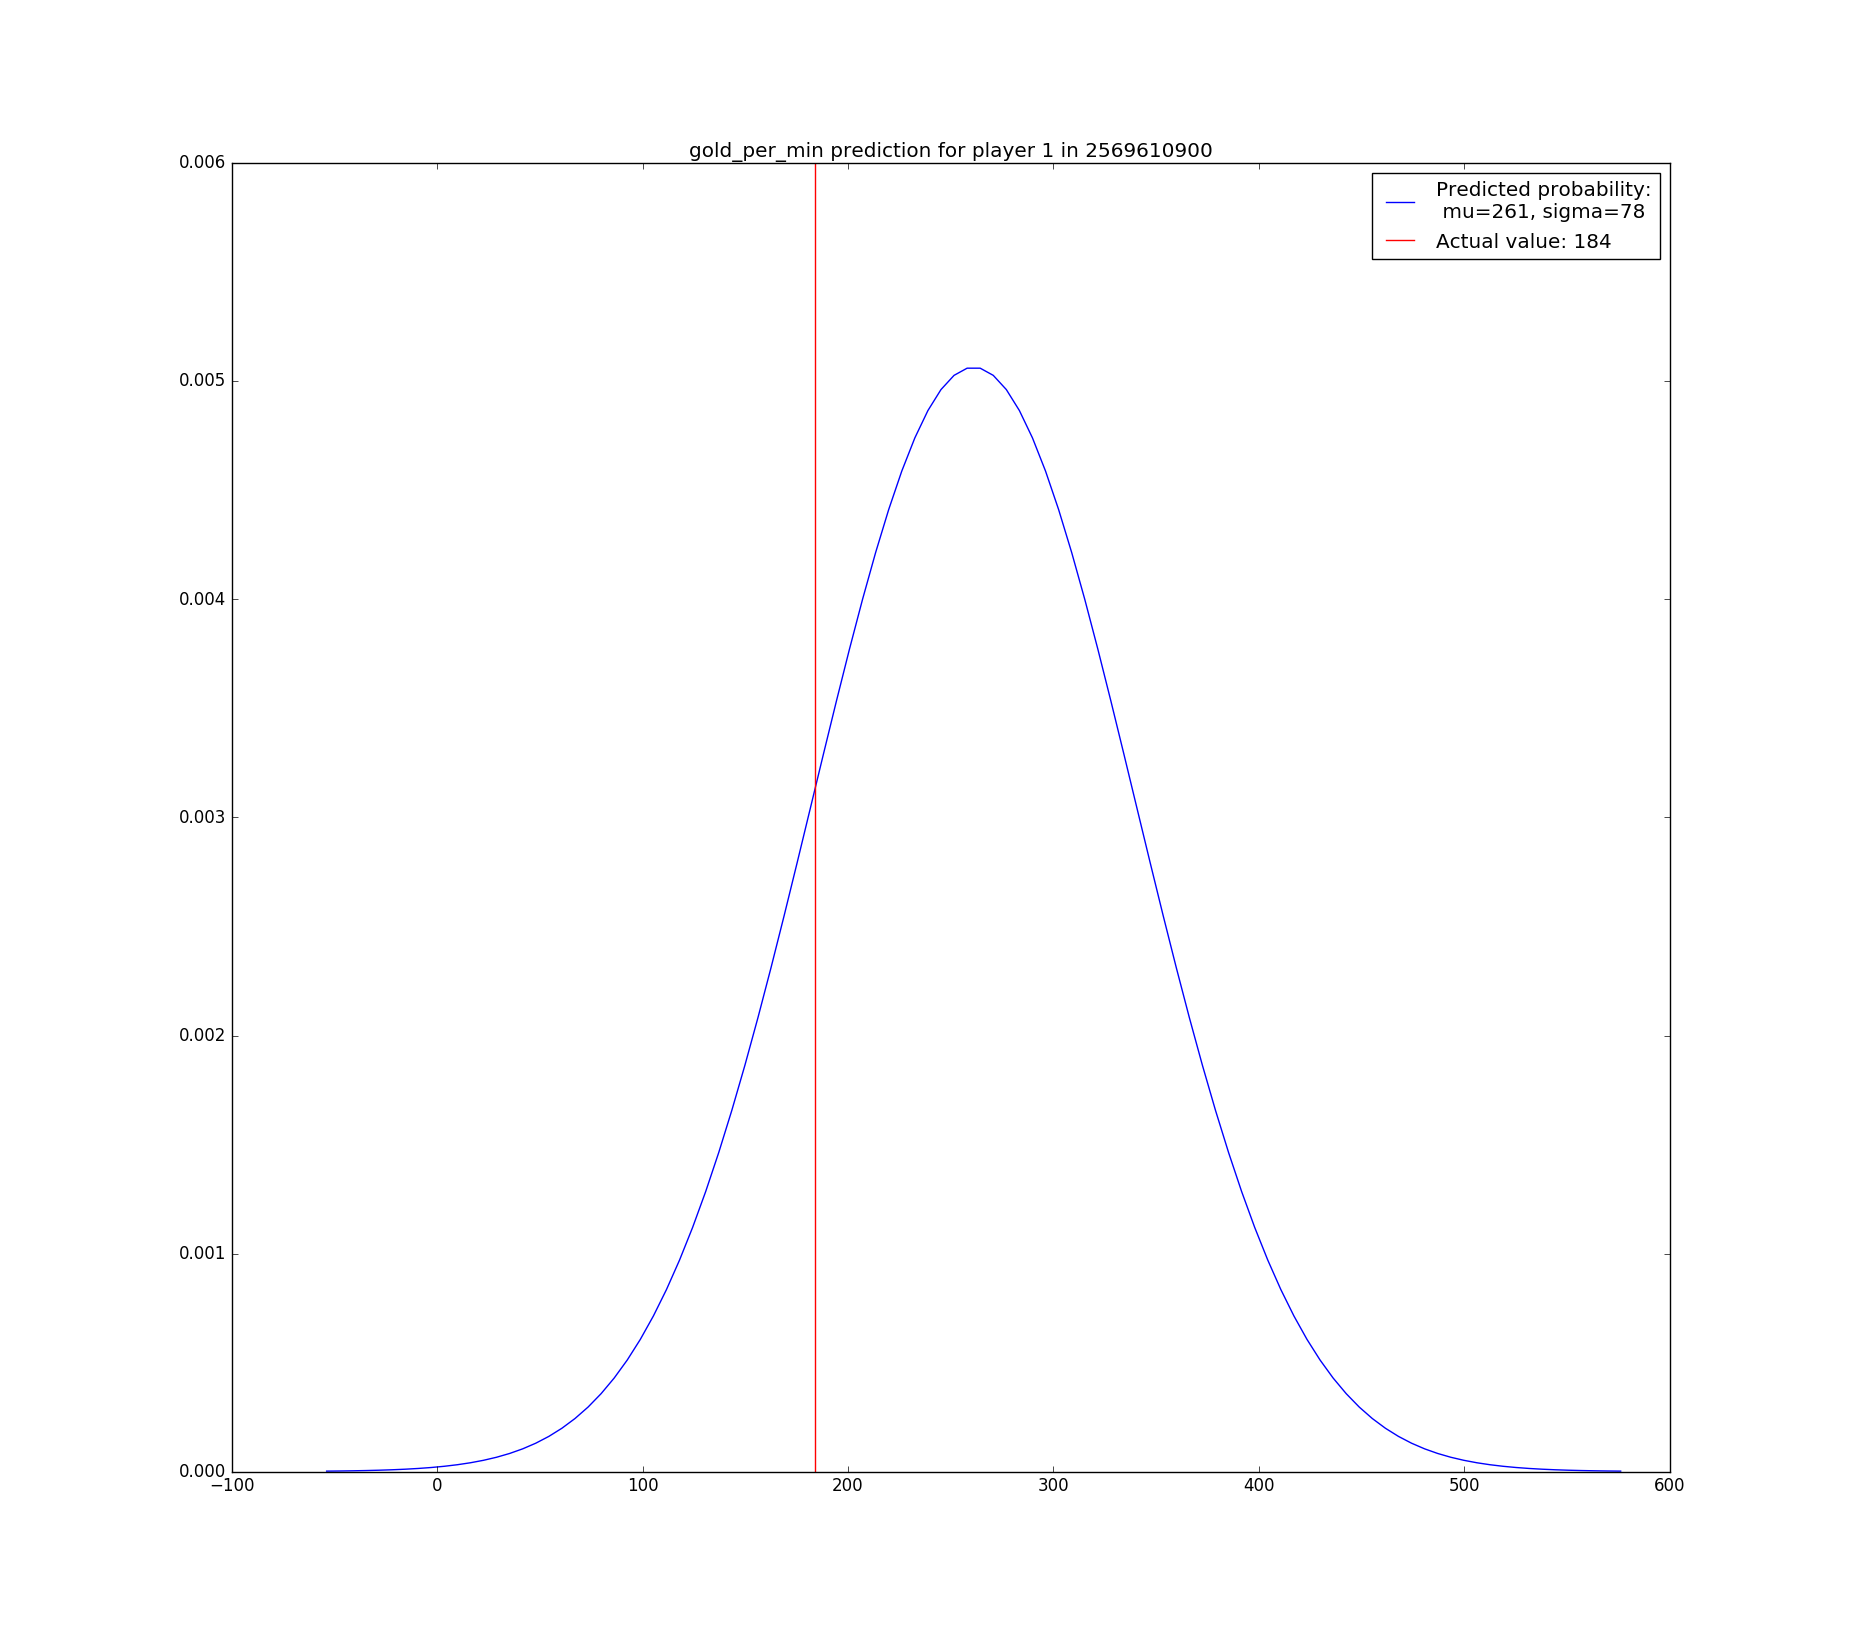
\includegraphics[width=5cm,height=4cm]{GPM_player_1_TI}
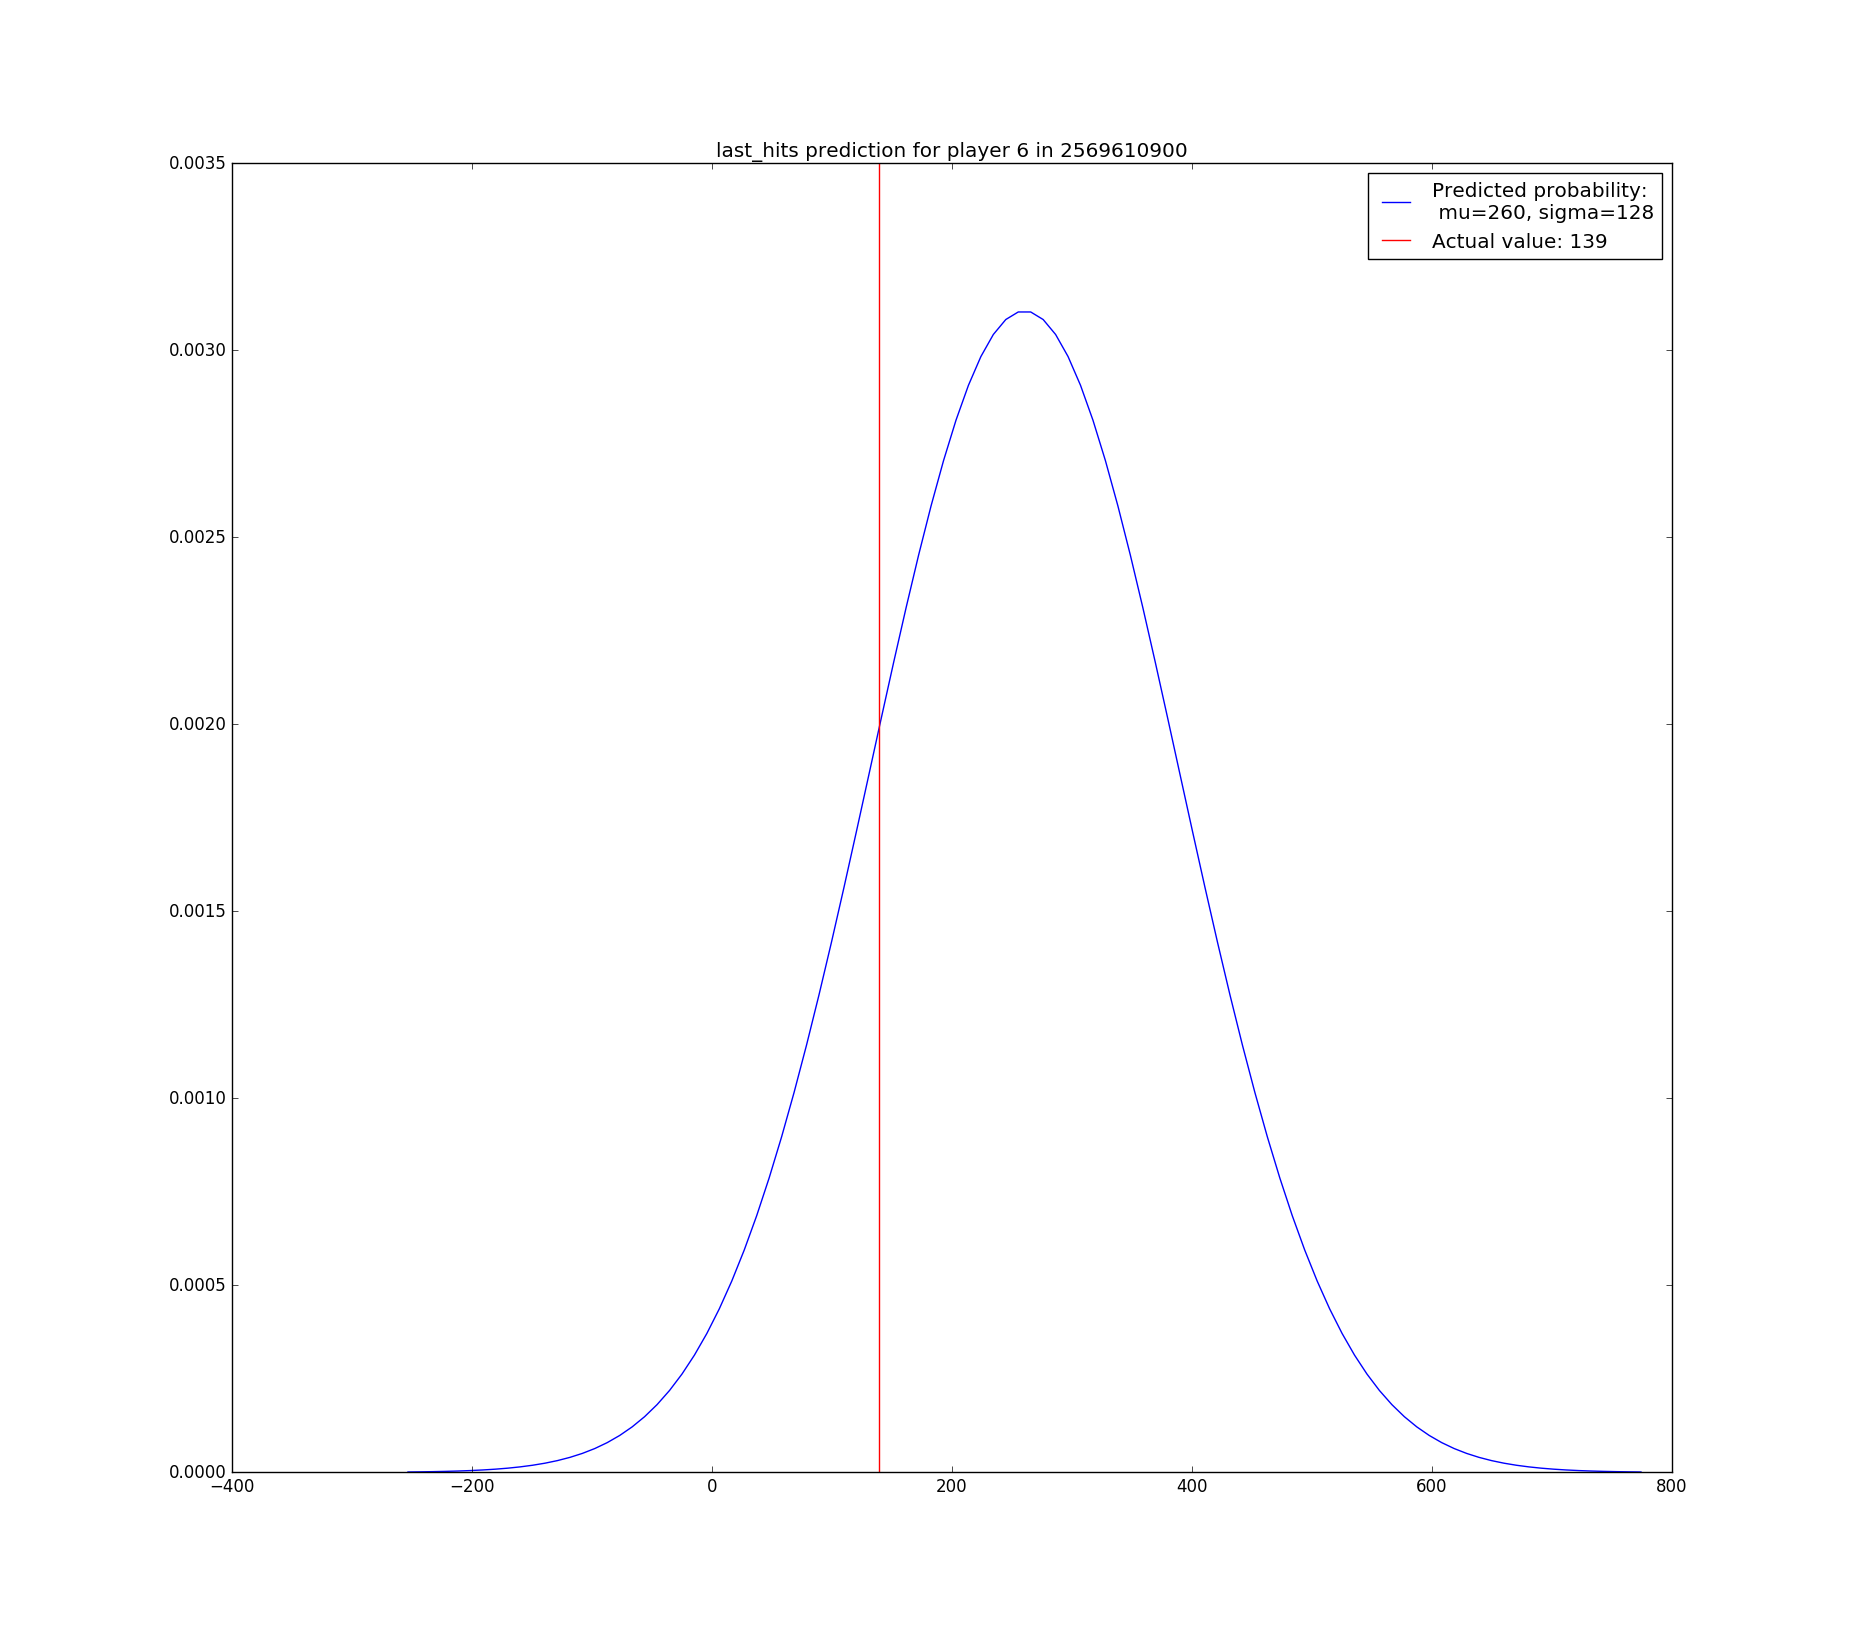
\includegraphics[width=5cm,height=4cm]{CS_player_6_TI}
\end{center}
\end{frame}

\end{document}
